\documentclass[12pt]{article}

\usepackage{epsfig,a4wide,amsmath,amssymb,amsfonts,mathrsfs}
\usepackage{ulem}

\usepackage[colorlinks=true]{hyperref}
\usepackage{enumitem}

\pagestyle{headings}

\newcommand{\du}{\mathrm{d}}

\setlength{\textwidth}{17cm}
\setlength{\oddsidemargin}{-0.4cm}
\setlength{\topmargin}{0.0cm}
\setlength{\textheight}{22cm}
\setlength{\parindent}{0.5cm}

\numberwithin{equation}{section}

\renewcommand{\textfraction}{0}
\renewcommand{\topfraction}{1}
\renewcommand{\floatpagefraction}{1}

\newcommand*{\defeq}{\mathrel{\vcenter{\baselineskip0.5ex \lineskiplimit0pt
                     \hbox{\scriptsize.}\hbox{\scriptsize.}}}%
                     =}
\newcommand*{\invdefeq}{=\mathrel{\vcenter{\baselineskip0.5ex \lineskiplimit0pt
                     \hbox{\scriptsize.}\hbox{\scriptsize.}}}%
                     }
\newcounter{count}

\normalem

\title{Notes on boson stars in scalar-tensor theory and code infrastructure}
\author{Tamara Evstafyeva}
\date{}
\begin{document}
\maketitle
% \tableofcontents
\newpage

%=============================================================================
\section{Variables}
To avoid confusion, I have mainly used the variables of Uli's notes, i.e.
\begin{itemize}
    \item $A$ -- amplitude of the bosonic scalar field.
    \item $\omega$ -- frequency of the boson star, in the code we start with initial guess of $\omega =1$, but this can be changed if searching for other solutions.
    \item $\varphi$ -- gravitational scalar field.
    \item $\alpha$ -- lapse function.
    \item $X$ -- function of $r$ from line-element ansatz $\du s^2 = -\alpha^2 \du t^2 + X^2 \du r^2 + \frac{r^2}{F} \du \Omega^2$.
    \item $W(\varphi)$ -- potential function for the gravitational scalar field given by $W(\varphi) = \frac{1}{2}\mu_{\varphi}^2 \varphi^2$, where $\mu_{\varphi}^2$ is the mass variable.
    \item $V(A^2)$ -- solitonic potential for the bosonic scalar field defined by $V(A^2) = A^2\left(1 - 2\frac{A^2}{\sigma_0^2}\right)^2$.
    \item $F(\varphi)$ -- conformal factor defined by $F(\varphi) = e^{-2\alpha_0 \varphi-\beta_0\varphi^2}$.
\end{itemize}
To have only first order derivatives, we further introduce the following auxiliary variables
\begin{align}
    \partial_r \varphi &= X \eta, \\
    \partial_r A &= \Psi_0.
\end{align}
We also choose to use $\Phi$ instead of the lapse $\alpha$, which is defined as
\begin{equation}
    \Phi = \rm{ln} \left(\sqrt{F} \alpha \right).
\end{equation}
Finally, we note that
\begin{equation}
    \frac{\partial_r F}{F} = \frac{F_{, \varphi}}{F}\partial_r \varphi = \frac{F_{, \varphi}}{F}X \eta.
\end{equation}


%=============================================================================
\section{Equations of integration}
Below we detail the equations that we implement for outward integration in the code. Note that the set of variables we are solving for is given by $\{\Phi, X, \eta, \Psi_0 \}$.
\begin{eqnarray}
  \partial_r \Phi
  &=&
  \frac{FX^2-1}{2r}
  -rFX^2W
  +\frac{r}{2}(X \eta)^2
  +2\pi r\frac{X^2}{F}\left[
  \frac{\Psi_0^2}{X^2}
  +\frac{A^2 \omega^2}{\alpha^2}
  -V
  \right]\,,
  \label{eq:Phir}
  \\[10pt]
  \frac{\partial_r X}{X}
  &=&
  -\frac{FX^2-1}{2r}
  +rFX^2W
  -\frac{1}{2}\frac{F_{, \varphi}}{F} X \eta
  +\frac{r}{2}(X \eta)^2
  +2\pi r\frac{X^2}{F}
  \left[
  \frac{\Psi_0^2}{X^2}
  +\frac{A^2 \omega^2}{\alpha^2}
  +V
  \right]\,,
  \label{eq:Xr}
  \\[10pt]
  \partial_r \eta
  &=&
  -\eta \left(
  \partial_r \Phi
  -\frac{1}{2} \frac{F_{, \varphi}}{F} X \eta
  \right)
  -\frac{2}{r}\eta
  + FX^2 W_{,\varphi}
  +\frac{2\pi XF_{,\varphi}}{F^2}
  \left[
  \frac{A^2\omega^2}{\alpha^2}
  -\frac{\Psi_0^2}{X^2}
  -2V
  \right]\,,
  \label{eq:etar}
  \\[10pt]
  \partial_r \Psi_0 &=&
  -2\frac{\Psi_0}{r}
  +\Psi_0 \left(
  \frac{\partial_r X}{X}
  + \frac{3}{2}\frac{\partial_r F}{F}
  - \partial_r \Phi
  \right)
  - \frac{X^2\omega^2 A}{\alpha^2}
  + X^2V_{\,,|\psi|^2} A\,,
%  - \frac{X^2\omega^2 \textcolor{red}{A} \cancel{A^2}}{\alpha^2}
%  + \textcolor{red}{X^2V_{\,,|\psi|^2} A}\cancel{X^2V_{\,|\varphi|^2} A}\,.
  \label{eq:Psi0r}
\end{eqnarray}
where I was lazy to replace $\alpha \rightarrow e^{\Phi}/\sqrt{F}$.

%=============================================================================
\section{Boundary conditions at the origin}
At $r = 0$, the boundary condition are
\begin{align}
    &\partial_r \varphi (r = 0) = 0 \implies \eta(r = 0) = 0, \\
    &\partial_r A (r = 0) = 0, \\
    &\Phi(r = 0) = 1, \\
    &A(r = 0) = A_{\rm{c}} \quad \text{(user-specified)}, \\
    &X(r = 0) = \frac{1}{\sqrt{F(\varphi(0))}}, \\
    &\varphi(r = 0) = \varphi_{\rm{c}} \quad \text{(user-specified but is checked and improved until surface condition is satisfied)}.
    \label{eq:bcsattheorigin}
\end{align}

%=============================================================================
\section{Series expansion near the origin}
Using the boundary condition at the origin \eqref{eq:bcsattheorigin}, we are able to derive the behaviour of our PDEs at the origin, which in the code are implemented within an open ball of small radius ($r_{\rm{small}} = 10^{-15}$)
\begin{align}
    \partial_r \Phi &= 0, \\
    \partial_r X & = 0, \\
    \partial_r \Psi_0 &= \frac{1}{3} \left(\frac{1}{F} V_{\,,|\psi|^2} A - \omega^2 A e^{-2 \Phi} \right), \\
    \partial_r \eta & = \frac{1}{3} \left[\sqrt{F({\varphi(0))}} W_{, \varphi} + \frac{2 \pi F_{, \varphi}}{F^2 \sqrt{F}}
     \left(\frac{\omega^2 A^2 F}{e^{2 \Phi}} - 2V \right) \right].
\end{align}

%=============================================================================
\section{Asymptotic behaviour}
Whilst the asymptotics turned quite out tricky and we have identified 3 cases that should be analysed separately for when $\alpha_0 \neq 0$ (with 2 of them being 'physical'). We focus on the case when $h < 2k$, which forces most of the 'nasty' terms to cancel in the asymptotic behaviour of the equations. This means the asymptotic behaviours of the bosonic scalar field and the gravitational scalar field are summarized as follows
\begin{align}
    A & \sim \frac{e^{-hr}}{r^{1+\delta}}, \quad \text{where} \quad h=m \quad \text{and} \quad \delta = Mm = Mh, \\
    \varphi & \sim \frac{e^{-kr}}{r^{1+\epsilon}}, \quad \text{where} \quad k=\sqrt{1-\omega^2} \quad \text{and} \quad \epsilon = M\frac{1-2\omega^2}{k} = M\frac{2k^2-1}{k},
\end{align}
where we estimate the mass $M$ using the mass function $m(r) \defeq \frac{r}{2} \left(1-\frac{1}{FX^2}\right)$ and the frequency $\omega$ through the shooting algorithm. It is crucial to note that we also need to reinforce that the lapse function goes to unity at infinity, that is $\lim_{r \to \infty} \alpha = 1$. We can re-scale $\alpha$ (or $\Phi$ in our case), as long as we re-scale $\omega$ with it! This is achieved via $\omega \rightarrow \omega e^{-\rm{ln}(\sqrt{F}X) -\rm{ln}(\sqrt{F}\alpha)}$.

%=============================================================================
\section{Methodology}
The idea is pretty much the same as for our 'classic' boson stars. Briefly, this means that we take our equations \eqref{eq:Phir}--\eqref{eq:Psi0r} and integrate them outwards until some $r_{stop}$, where the solution for the bosonic field diverges and goes bonkers. From $r_{stop}$ we set the bosonic variable counterparts to zero to avoid crashing the code. We then find the minimum of the bosonic scalar field before it starts to diverge, and glue the asymptotic behavior to it. 

We concentrate on the \textit{massless} case for the time being, and in this case we do not use the asymptotic behavior for $\varphi$, as it is super slow, but rather just continue integrating outwards the equation for the gravitational scalar field. We repeat the whole integration from the point of asymptotic matching, now hopefully getting a physical solution. 

Usually any initial guess for $\varphi_{\rm{c}}$ produces something. However, is it what we are looking for? Sadly, not really. To enforce 'the correct solution' in the code, we use the surface condition equation for the gravitational scalar field by Damour \cite{Damour:1993hw, Gerosa:2016fri}. It is in principle applicable to vacuum, however far away (at large radius) the boson star is fairly 'vacuum', we assume it is an alright for us approximation to use. The condition gives the expected value for the gravitational scalar field on the surface of the star, or just 'far enough' for our case
\begin{equation}
    \varphi_{\rm{s}} = - \frac{X_{\rm{s}} \eta_{\rm{s}}}{\sqrt{(\partial_r \Phi_{\rm{s}})^2 + X_{\rm{s}} \eta_{\rm{s}}}} \rm{artanh} \frac{\sqrt{(\partial_r \Phi_{\rm{s}})^2 + X_{\rm{s}} \eta_{\rm{s}}}}{\partial_r \Phi_{\rm{s}} + 1/r_{\rm{s}}}.
\end{equation}
Here by 's' we denote the variable evaluated on the star's surface. In our code the surface is defined as just a few gridpoints away from the edge of the grid. We quantity how well this condition is satisfied by comparing it with our numerical value for $\varphi$ at that surface point, and improve on the central field guess $\varphi_{\rm{c}}$ until we meet this surface condition up to some satisfactory tolerance (i.e. $10^{-5}$) using Newton-Raphson algorithm.

\section{Some solutions: massless case}
A bit on the pessimistic side, but I decided to start with \textit{very} negative value for $\beta_0$, which is $\beta_0 = -12.0$. For those interested other parameter values has been set to $\alpha_0 = 0.01$ and $A_{\rm{c}} = 0.147$.

\begin{figure}
    \centering
    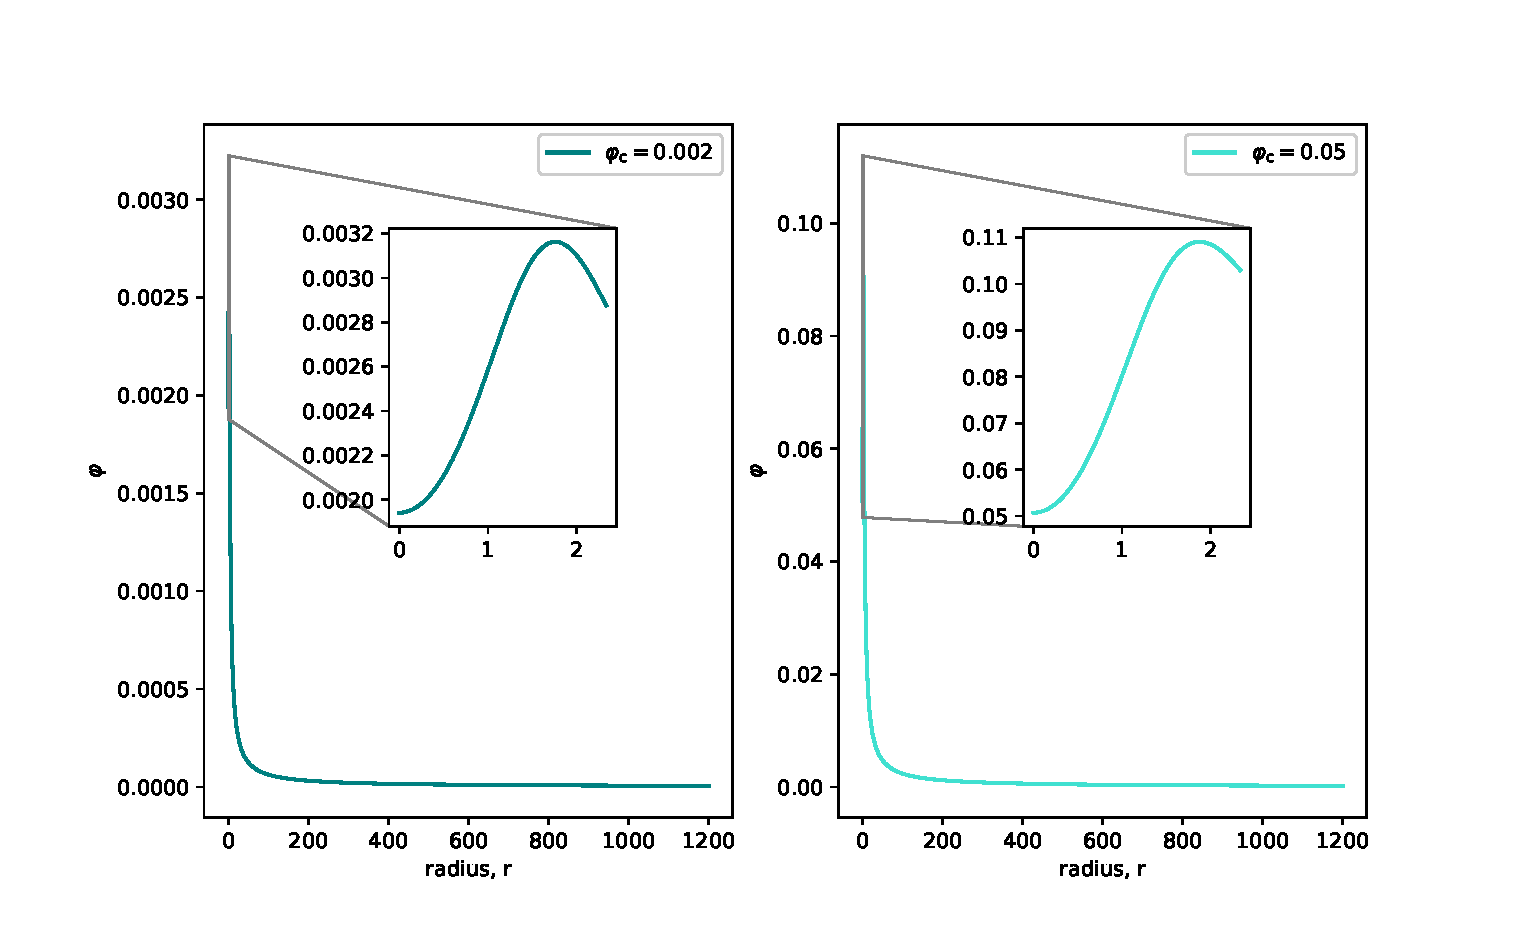
\includegraphics[width=15cm]{model-beta-12.eps}
    \caption{Profile of the gravitational scalar field as a function of the radius, computed from different initial guesses for $\varphi_{\rm{c}}$. One yields a profile of roughly $\mathcal{O}(\alpha)$, whereas the other one results in much more scalarisation giving $\varphi \sim \mathcal{O}(1)$; the asymptotic condition is satisfied for both cases.}
    \label{model-beta-12.eps}
\end{figure}

%============================================================================
\bibliographystyle{unsrt}
\bibliography{biblist}

\end{document}
